\section{Datatset}
\label{sec:dataset}
Particular attention is needed in the construction of a good training dataset, 
in fact, as seen before in (\ref{subsec:supervised-learnig}), we deal with a
supervised learning where we know the response of our labels and bounding box
positioned objects. A script is provided that can build a dataset divided into
folders: training, validation and testing; as you can see in figure
(\ref{fig:datasetstructure}).
A large number of figures per sample that clearly highlight the characteristics
that you want to study allows a greater rate of success of the training
preventing the \emph{overfitting}.
Acquiring a large number of images is not always achievable, using some
augmentation techniques, which virtually allow to increase the observability of
images, for example, by rotating, distorting and translating them. 
The two train and validated folders are essential for the addition of the neural
network. Instead, the test folder contains a set of images that the network has
never seen and so it is necessary to measure the degree of confidence acquired
in the network.\linebreak
%
\begin{figure}[htb]
	\centering
	\includegraphics[width=0.75\textwidth]{structure.jpg}
	\caption{Dataset structure}
	\label{fig:datasetstructure}
\end{figure}
%
\subsection{Landing zone dataset}
\label{ssec:landing-zone}
%
The dataset was artificially constructed with a 3D Blender graphics program.(\ref{fig:blender})\\ 
The object of interest are the drone landing mats. These have different shapes
and colors in fact they are available in various color shapes. The signs on
these also vary from the classic H to X to more or less conspicuous symbols.
Thus three models were created, two with a circular plan and one with a square
plan. 
Textures were then applied to these two models to obtain a faithful
representation of that of concrete objects. \hfill \break
After the construction of the carpet models, it was necessary to contextualise 
them in credible scenarios.\hfill \break
%
\begin{figure}[htb]
	\centering
	\includegraphics[width=0.75\textwidth]{blender.jpg}
	\caption{Modelling phase of the scenario in Blender.}
	\label{fig:blender}
\end{figure}
%
\\Thus, three main scenarios were created: first scenario placed in the middle of a road
junction. Second scenario near a straight road flanked by a side-walk.
Third zone is set in the countryside. To take the shots, some photographic
factors were taken into account, in fact they are generated starting from the
technical characteristics of the Raspberry camera presented in section
(\ref{sec:raspicam}). Moreover, thanks to a simple script, the trigger points
were generated with respect to the landing mat position, these positions vary in
height, width and depth with respect to the carpet placed on the ground.\\
A scheme is visible in figures (\ref{fig:poi_dataset}). \hfill \break
%
\begin{figure}[htb]
	\centering
	\includegraphics[width=0.75\textwidth]{poi_dataset.jpg}
	\caption{Configuration camera position.}
	\label{fig:poi_dataset}
\end{figure}
%
\newpage
To increase the variety of rendered shots, a very basic day-night cycle was
used to detect the color variation. All the shots are taken with a top view as
seen in the examples shown in (\ref{fig:renders}).
After completing the shots they annotated themselves highlighting the position
of the object of interest in the various shots and positions.\\
The process is carried out with the aid of a software that extracts and
generates the annotations. As shown in figure (\ref{fig:annotation}).
\begin{figure}[htb]
	\centering
	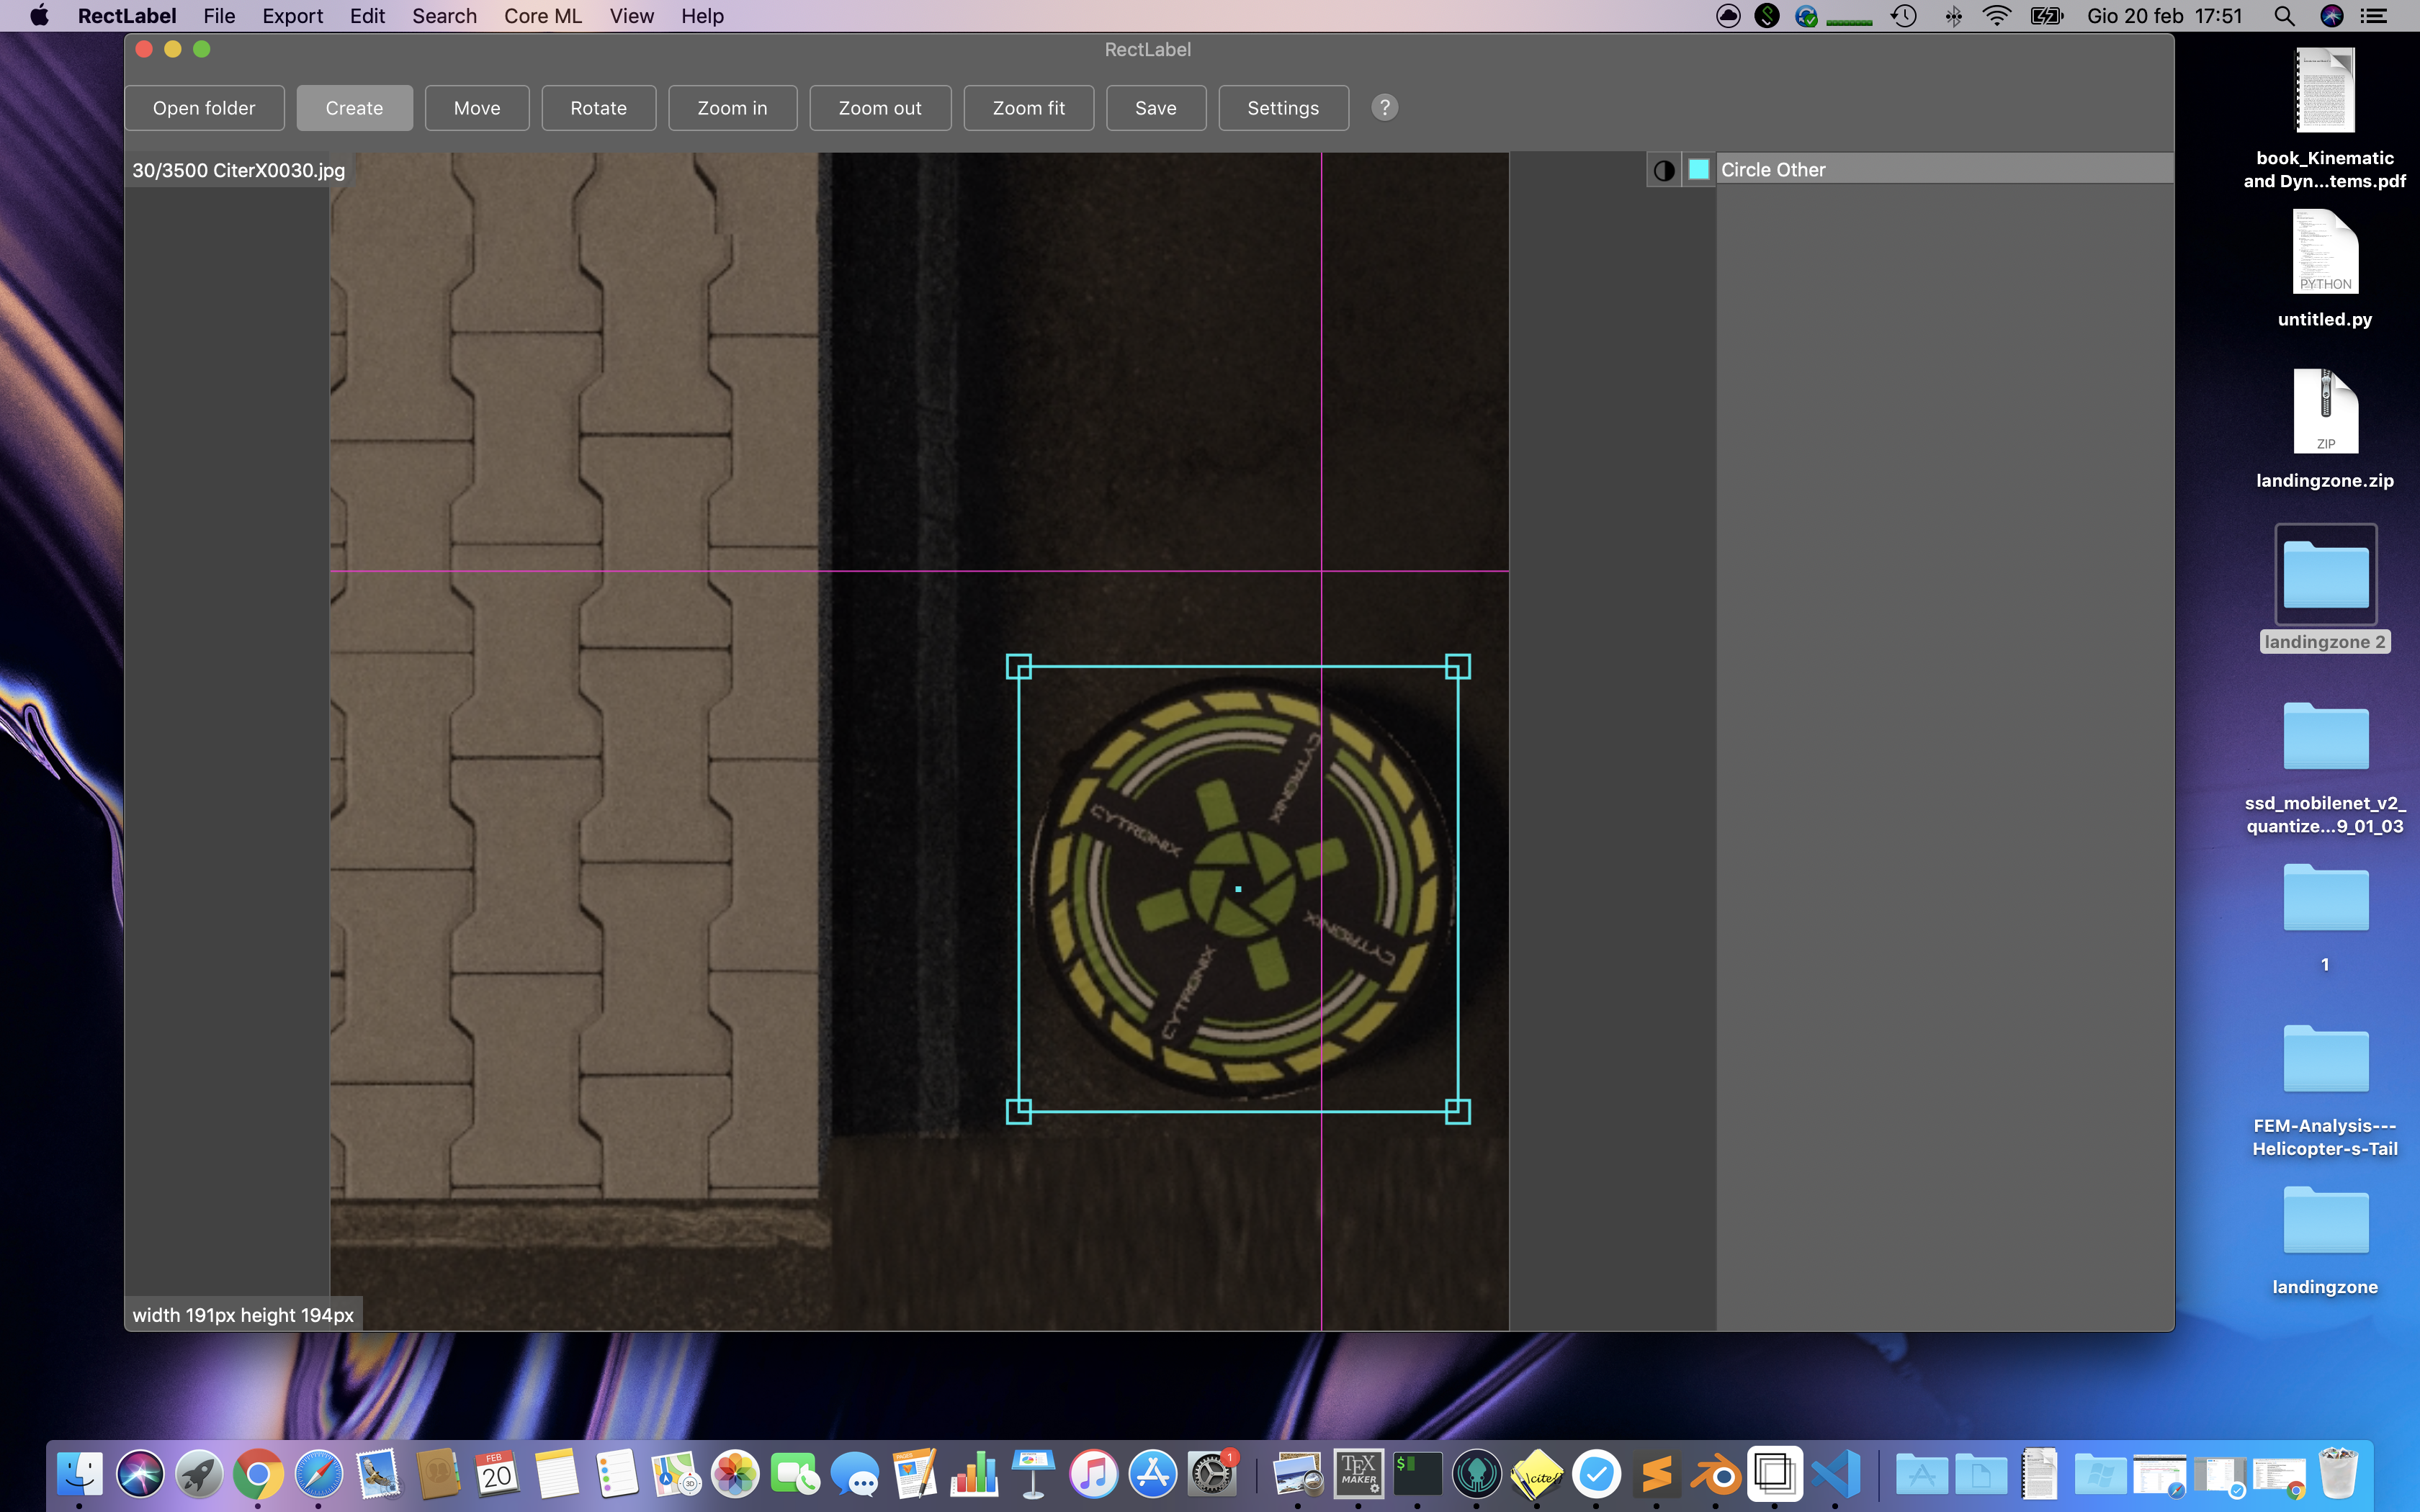
\includegraphics[width=0.70\textwidth]{annotation.jpg}
	\caption{Process of annotation.}
	\label{fig:annotation}
\end{figure}
%
\begin{figure}[htb]
    \centering
    \subfloat[][\emph{middle of a road junction (sunrise)}.\label{subfig:junction}]
        {\includegraphics[width=.50\textwidth]{result1.jpg}} \quad
    \subfloat[][\emph{countryside}.\label{subfig:country}]
        {\includegraphics[width=.50\textwidth]{result2.jpg}} \quad
    \subfloat[][\emph{close position at the crossroads}.\label{subfig:junction2}]
        {\includegraphics[width=.50\textwidth]{result3.jpg}}
    \caption{Examples shots scenarios after render}
    \label{fig:renders}
\end{figure}
%
%
\subsection{Thermal imaging dataset}
\label{ssec:thermal-image-dataset}
The dataset created and distributed free of charge by
FLIR\footnote{\href{https://www.flir.com/oem/adas/adas-dataset-form/}{https://www.flir.com/oem/adas/adas-dataset-form/}}
was used to train the neural network on the recognition and classification of
objects in thermal images. The ability to sense thermal infra-red radiation, or
heat, within the ADAS context provides both complementary and distinct
advantages to existing sensor technologies such as visible cameras, LiDAR and
radar systems: With over 15 years of experience in automotive, FLIR has the only
automotive-qualified thermal sensor that is deployed in over 500,000 cars today
for driver warning systems. The FLIR thermal sensors can detect and classify
pedestrians, bicyclists, animals and vehicles in challenging conditions
including total darkness, fog, smoke, inclement weather and glare, providing a
supplemental dataset beyond LiDAR, radar and visible cameras. The detection
range is four times farther than typical headlights. When combined with visible
light data and distance scanning data from LiDAR and radar, thermal data paired
with machine learning creates a more comprehensive detection and classification
system.\cite{flirdataset}\hfill\break
\\The dataset provided by FLIR was created from videos collected from a moving
vehicle in Santa Barbara, California, USA covering roads and highways in
different weather conditions. Although there are many objects in the images to
be catalogued, only ten types of objects have been selected, in particular:
\begin{itemize}
\item Category 1: People
\item Category 2: Bicycles - bicycles and motorcycles (not consistent with coco)
\item Category 3: Cars - personal vehicles and some small commercial vehicles.
\item Category 17: Dogs
\end{itemize}
%
The boxes around the objects of interest are as narrow as possible in fact: when
occlusion occurred, only non-occluded parts of the object were annotated. Heads
and shoulders were favoured for inclusion in the bounding box over other parts of
the body for people and dogs. When occlusion allowed only parts of limbs or
other minor parts of an object to be visible, they were not annotated. 
Wheels were the important part of the Bicycles category.
Bicycle parts typically occluded by riders, such as handlebars, were not included in the bounding box.
People riding the bicycle were annotated separately from the bicycle. When an
object was split by an occlusion, two separate annotations were given to the two
visible parts of the object.
%
\begin{figure}[htb]
    \centering
    \subfloat[][\emph{person}.\label{subfig:th-person}]
        {\includegraphics[width=.50\textwidth]{FLIR_00658.jpeg}} \quad
    \subfloat[][\emph{cars and people}.\label{subfig:th-car}]
        {\includegraphics[width=.50\textwidth]{FLIR_00690.jpeg}} \quad
    \subfloat[][\emph{bicycle and persons}.\label{subfig:th-bycicle}]
        {\includegraphics[width=.50\textwidth]{FLIR_00356.jpeg}}
    \captionsource{Thermal image extracted from FLIR dataset.}{\href{https://www.flir.com/oem/adas/adas-dataset-form/}{https://www.flir.com}}
    \label{fig:th-image}
\end{figure}